			\documentclass{article}
			\usepackage{graphicx}
			\usepackage{listings}
			\usepackage{titlepic}
			\usepackage{float}
			\usepackage{hyperref}
			\newcommand\tab[1][1cm]{\hspace*{#1}}
			\newcommand{\quotes}[1]{``#1''}
			\usepackage{multicol}
			\renewcommand{\labelenumii}{\theenumii}
			\renewcommand{\theenumii}{\theenumi.\arabic{enumii}.}
			
			\begin{document}
			\title{
\includegraphics[scale = .6]{uom.png}
				\linebreak 
				\textbf{CPS2000 - Compiler Theory \& Practise}\linebreak\linebreak
				\textbf{Assignment Part 1}\linebreak\linebreak
				\large{B.Sc Computer Science}
				\date{}
				\author{Jacques Vella Critien - 97500L}}
				
				\begin{titlepage}
					\maketitle
					\thispagestyle{empty}
				\end{titlepage}
				
				\tableofcontents
				\newpage
				
				\section{Task1: Boolean Satisfiability}
				
				In this task, we were required to write a command line program that accepts Boolean expressions in Conjunctive Normal Form (CNF). Moreover, this implementation should:
				
				\begin{itemize}
				\item accept symbols \quotes{w}, \quotes{x}, \quotes{y} and \quotes{z} to represent literals
				\item use the \quotes{!} symbol to represent negation
				\item use parenthesis to group clauses
				\item use commas	to	separate literals	in	clauses
				\item white-space is irrelevant and should be ignored while parsing
				\end{itemize} 
				
				\noindent Moreover, the Davis-Putnam-Logemann-Loveland (DPLL) algorithm had to be implemented to determine whether the expression is satisfiable. If the expression is satisfiable the program should display a truth assignment as a proof, while if it is unsatisfiable, the program should display \quotes{UNSAT}.\\
				
\noindent Finally, we are to dedicate a section to describe the practical applications of SAT. 

		\subsection{Solutions}
		
		\subsubsection{SyntaxErrorException.java}
		
		This is an exception thrown when there is something wrong with the string passed to be parsed by the parser
		
		
		\subsubsection{Assignment.java}
		
		This is an enum to hold the assignment value and this can be either TRUE, FALSE or DONTCARE.
		
		\subsubsection{Symbol.java}
		
		The assignment states that the implementation should include the values  \quotes{w}, \quotes{x}, \quotes{y} and \quotes{z} but in this enum class which contains the different symbols available for literals or variables, I also added  \quotes{v} for more testing.
		
		\subsubsection{Literal.java}
		
		This is a class which represents a literal. It has the following member variables:
		\begin{itemize}
		\item \textbf{negated}: This is a boolean to hold if the literal is negated or not
		\item \textbf{symbol}: This is of type Symbol explained above and is used to hold the symbol or type of the literal.
		\end{itemize}
		
		In addition, this class consists of the following methods
		
		\begin{enumerate}
		\item \textbf{Literal(String)}: This is a constructor that when given a string it initialises the literal object from it. This is done by first checking if the length of the string passed is greater than 2 or if the length is 2 and that the first character is 2. If so, it means that the string passed is not of the correct format, therefore a \textbf{SyntaxErrorException} is thrown. Otherwise, it is checked whether the passed literal is negated by checking if the size is 2, if so meaning that it is negated and if not, it means that the literal is not negated. The last step involves obtaining the symbol of the literal from the string and setting it. In case of a symbol different from the accepted ones, a \textbf{SyntaxErrorException} is thrown.
		
		\item \textbf{isNegated()}: This is a getter for the negated member variable.
		\item \textbf{setNegated(boolean)}: This is a setter for the negated member variable.		
		\item \textbf{getSymbol()}: This is a getter for the symbol member variable.
		\item \textbf{setSymbol(Symbol)}: This is a setter for the symbol member variable.	
		\item \textbf{equals(Literal)}: This is a method to check if the current literal is equal to the one passed. This is done by checking if both literals contain the same symbol and negation.
		\item \textbf{clone()}: This is a method to clone a literal, i.e., getting its values, setting them to a new Literal object and returning it.
		
		\end{enumerate}
		
		\subsubsection{Clause.java}
		
		This is a class which represents a clause. It has the following member variable:
		\begin{itemize}
		\item \textbf{literals}: This is an arraylist of Literals, used to hold the literals in the clause.
		\end{itemize}
		
		In addition, this class consists of the following methods
		
		\begin{enumerate}
		\item \textbf{Clause(ArrayList\textless Literal\textgreater)}: This is a constructor that when given an array-list of literals, they are set to member variable holding literals.
		
		\item \textbf{Clause()}: This is an empty constructor for clause and it just initialises the array-list of literals.
		\item \textbf{getLiterals()}: This is a getter for the literals member variable.		
		\item \textbf{addLiteral(Literal)}: This is a function which just adds a literal to the array-list holding literals.
		
		
		\end{enumerate}
		
		\subsubsection{Parser.java}
		
		This is the class used to represent the parser, hence which turns boolean expressions as strings and parses them into objects of clauses and literals. Moreover, this performs error checking to make sure that these expressions are entered in the correct format. 
		
		This class contains the following methods:
		
			\begin{enumerate}
		\item \textbf{parseString(String)}: This function is the main function used to parse a string into proper objects of clauses and literals by returning a set of clauses\\
		This is done by first checking making sure that the string is not empty and if so a \textbf{SyntaxErrorException} is thrown. The next step involves removing all white-spaces before checking whether the first character of the string is a `(` and the last character of the string is a `)` and if not, a \textbf{SyntaxErrorException} is thrown.\\\\
		After these checks, the parsing starts by removing the first and last characters which should be `(` and a `)` and then create a string tokenizer with the delimeter set to `)(` so that each clause is seperated. The next step involves going through each token stored by the clause tokenizer and for every token, a new clause object is created and each literal is obtained by creating another tokenizer, this time operating with the delimeter set to `,`. Before moving to the next step, it is worth mentioning that, the DPLL class, which will be explained in the next section, contains a member variable of type hashmap with the a Symbol key and an Assignment enum value as value, called \textbf{assignments} to hold assignments, i.e. every literal symbol being used in the clause. \\\\
		After this, for every literal in each clause, a new Literal is created by calling the literal constructor accepting a string and if the \textbf{assignments} map does not contain the symbol, the symbol is added to the list with a DONTCARE assignment. Finally, the literal is added to the clause created in the loop containing the clauses and once all the literals of the clause are iterated through, the clause is added to the set of clauses to be returned. \\\\
		After all the literals and clauses are visited, the set of clauses which was filled is returned.
		
		
		\item \textbf{printParsed(Set\textless Clause\textgreater}: This function is used to print the passed set of clauses in a parsed way. This is done by creating an iterator on the set of clauses and for each clause, the literals are obtained and are printed. If these are negated, a `$\neg$` before the symbol is printed. The clauses and literals are also numbered to make it easier for the user to understand them, for an example, one can take a look at the figure below.
		
						\begin{figure}[H]
					\centering
			 			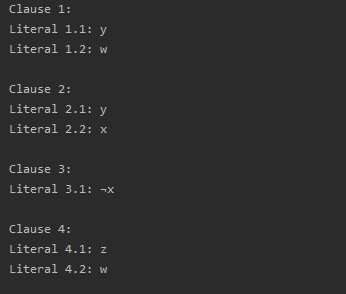
\includegraphics[width=0.55\textwidth]{printparsed.png}
			 			\centering
			  			\caption{Result for (!x)(y, x)(z,w)(y, w)}
			  			\label{fig:printparsed}
					\end{figure}
					
		
		\end{enumerate}
		
				\subsubsection{DPLL.java}
				
				This class contains methods for the DPLL algorithm and the actual DPLL function. 
				Moreover, this class has the following global variable:
		
		\begin{itemize}
		\item \textbf{assignments}: This is a hashmap with a key of type Symbol and a value of type Assignment. This variable is ought to hold each symbol found in the expression and keep its assignments so that if it is satisfiable, the assignments, computed on run-time can be easily displayed.
		\end{itemize}
				
	This class contains the following methods:
	
		\begin{enumerate}
		\item \textbf{removeTriviallySat(Set \textless Clause\textgreater)}: This method removes the trivially satisfiable, of the form (x, !x), clauses from the passed set of clauses and returns a set of clauses without the satisfiable clauses. In order to do this, a boolean flag named removed is held and an iterator is initiated based on the elements inside the passed set of clauses. 
		\\\\
		For every clause found in the iterator, removed is set to false, and the clause's literals are obtained. Apart from this, for every clause, there is an inner loop which goes through each literal in the clause until there is a removal or all literals have been iterated. Inside this loop, there is another nested loop to go through the literals one more time for comparison and if the literal of the outer loop and the literal of the inner loop are of the same symbol but their negation is different, hence in the form (x, !x), this clause is removed and removed is set to true. Finally, the remaining clauses are added. To help in the explanation the code snippet of this method can be found in the below image.
		
								\begin{figure}[H]
					\centering
			 			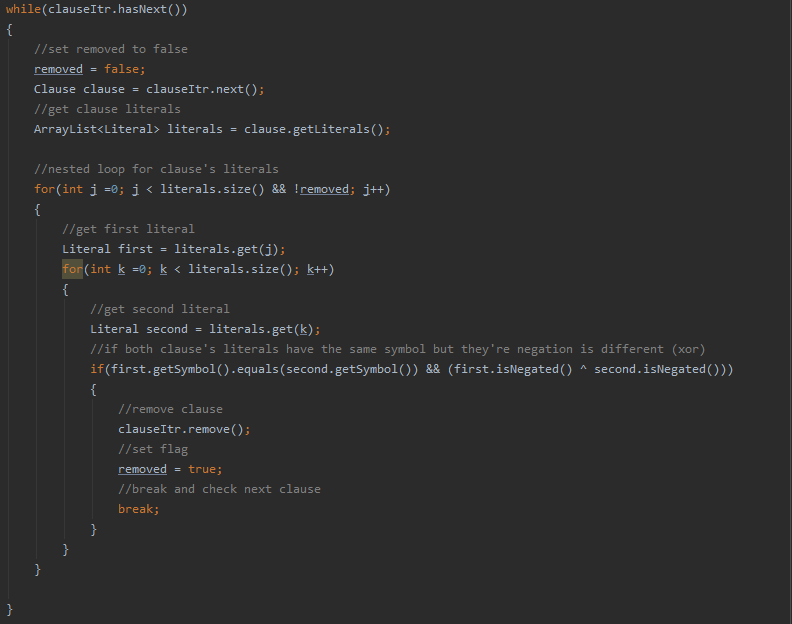
\includegraphics[width=0.8\textwidth]{removesat.png}
			 			\centering
			  			\caption{Code snipped for how to remove trivially satisfiable clauses}
			  			\label{fig:removesat}
					\end{figure}
		
		\item \textbf{checkTriviallyUnSat(Set \textless Clause\textgreater)}: This is a method which checks if there are any trivially unsatisfiable clauses, of the form (x)(!x), from a set of clauses. This is done by looping through all clauses and comparing them with each other.\\\\
		To do this, an iterator is used for the first loop which goes on until the iterator has another value. The first thing done in the first loop is to check if the the amount is literals inside the clause is 1 because if not, it cannot be an unsatisfiable clause, therefore, the loop proceeds to the next clause. Inside this loop, another iterator is obtained for the same clauses to compare and a nested loop is created to go through the clauses again.\\\\
		Inside the nested loop, the clause is obtained and the check for the amount of literals is done once again and if the size is not 1, this clause is skipped. If not, the literal from the first clause (outer loop) and the literal from the second clause (inner loop) are obtained. If these literals are of the same symbol and they have opposite negation, it must mean that they are of the form (x)(!x), hence, trivially unsatisfiable and true is returned. If no two clauses are found to be trivially unsatisfiable, false is returned.
		
		\item \textbf{checkEmptyClause(Set \textless Clause\textgreater)}: This is a function which checks if there are any empty clauses in the set of clauses passed as parameters. This is done by iterating through all the clauses and if the clause has no literal, true is returned.
		
		\item \textbf{getUnitClause(Set \textless Clause\textgreater)}: A unit clause is a clause containing only 1 literak, This is a function which returns a unit clause if there is one from the passed clauses and null if there is not. This is done by going through the clauses using an iterator and if the clause has only 1 literal, a copy of the clause is cloned and returned.
		
		\item \textbf{getPureLiteral(Set \textless Clause\textgreater)}: This is a function which returns a pure literal from the list of passed clauses. A pure literal is a literal which appears either positive or negative throughout all clauses. This is started by keeping a boolean flag named searching, initiating an arraylist of literals and adding all literals in all clauses in it. \\\\
		After this, there is a loop through all these literals. Inside this loop, the first thing we do is set the boolean flag searching to true and get the current literal. Then there a nested loop to go through the literals again for comparison and if the symbol from the first literal, is the same as the symbol from the literal in the nested loop and their negation is opposite, searching is set to false and we break out of the loop because it means that the outer literal is not pure. After the nested loop, there is a check for searching and if this is true, a clone of the literal in the outer loop is returned because it means that it is pure. If searching is always false, null is eventually returned.
		
				\item \textbf{exhaustivelyApply1LiteralRule(Clause, Set \textless Clause\textgreater)}: This is a function which given a unit clause and a set of clauses, returns a set of clauses after performing the 1 literal rule exhaustively on the passed set of clauses using the passed clause. \\
				
				This is done by looping through all clauses and doing the following:
				\begin{itemize}
				\item Getting current clause and its literals from iterator and getting the first literal from the passed unit clause
				\item Looping through each literal from the literals of the current clause and inside this loop:
					\begin{itemize}
						\item The current literal is obtained
						\item The unit clause literals negation value is inverted (so if it's not negated, negate it and vice-versa)
						\item If the current literal is equal to the unit clause inverted, the current literal is removed from the set of literals of its parent clause.
						\item The unit clause literal is re-inverted to its original negation
						\item It is checked if the current clause is equal to the unit clause and if so, the clause is removed and the loop is broken.

					\end{itemize}
				
					
				\end{itemize}
				
		Finally, the remaining clauses with their remaining literals are returned
	
		\item \textbf{applyPureLiteralRule(Literal, Set \textless Clause\textgreater)}: This is a function which returns a set of clauses after applying the pure literal rule exhaustively on the set of clauses passed using the passed pure literal. This is done by going through each clause in the passed clauses and then for each, clause there is another loop for each literal in this clause. If this literal is equal to the pure literal, the current clause in the loop is removed and the loop is broken. Finally the clauses are returned once all the clauses are traversed.
						
		\item \textbf{chooseLiteral(Set \textless Clause\textgreater)}: This function is a heuristic and from my research, I decided to implement it based on the \textbf{Dynamic Largest Individual Sum(DLIS)}, meaning that each literal is binned and the variable with maximal max(CP, CN) is selected, with CP and CN being the number of positive and negative occurrences. So this function, given a set of clauses, returns the most frequent literal. \\
		
		This is done by first initialising a hashmap with a key of type Literal and a value of type Integer, named bins to hold the number of occurrences. Then, the all the literals in all the clauses are stored in an arraylist and each literal from this arraylist is traversed and if the bins contained the literal, the value of the bin for that literal would be incremented, otherwise a new entry in the bin hashmap is created with the currently visited literal. After this, the maximum from the bins is obtained and a new literal with the symbol of the most frequent literal is returned.
		
		\item \textbf{DPLL(Set \textless Clause\textgreater)}: This function is the function that actually implements the Davis-Putnam-Logemann-Loveland algorithm which can be found below. This recursive function is passed a set of clauses and returns whether the boolean expression made up of the passed clauses is satisfiable.
		
					\begin{figure}[H]
					\centering
			 			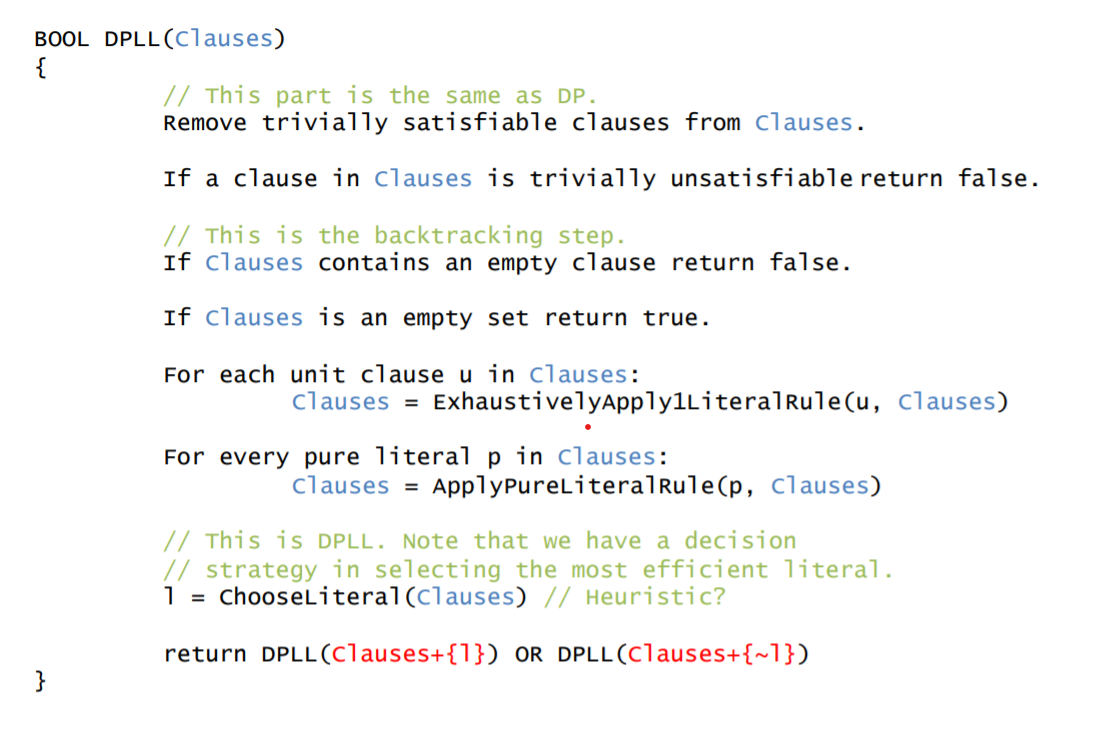
\includegraphics[width=0.7\textwidth]{dpllalgo.png}
			 			\centering
			  			\caption{DPLL algorithm from the notes}
			  			\label{fig:dpllalgo}
					\end{figure}
		
		This is done by first removing trivially satisfiable clauses by calling \textbf{removeTriviallySat()} with the passed clauses as parameters. Then, it is checked if there are any trivially unsatisfiable clauses by calling \textbf{checkTriviallyUnSat()} with the passed clauses as parameters and if so, `UNSAT` is printed and false is returned.
		Otherwise, it is checked if there are any empty clauses by calling \textbf{checkEmptyClause()} with the passed clauses as parameters and if so, \quotes{UNSAT} is printed and false is returned.
		Then, if not, it is checked whether clauses is empty because if this is the case, we can say that the boolean expression is satisfiable and therefore, the assignments stored in the assignments global variable are printed one by one and true is returned.\\\\
		The above were the base cases, and if none were reached, it means that we still have to perform some more operations before we get to know whether the expression is satisfiable or not. This is done by getting unit clauses one by one by calling \textbf{getUnitClause()} with the passed clauses as parameters and for each one, an assignment is set with the unit clause only literal's symbol as key and if it is negated the assignment is FALSE, otherwise, it is true. Moreover, for every unit clause, the 1-literal rule is applied exhaustively by calling \textbf{exhaustivelyApply1LiteralRule()} with the unit clause and clauses as parameters. \\\\
		The next step involves getting the pure literals one by one by calling \textbf{getPureLiteral()} with the passed clauses as parameters and for each one, an assignment is set with the pure literals's symbol as key and if it is negated the assignment is FALSE, otherwise, it is true. Moreover, for every pure literal, the pure literal rule is applied exhaustively by calling \textbf{applyPureLiteralRule()} with the pure literal and clauses as parameters. \\\\ 
		The final step involves getting a literal by calling the heuristic function \textbf{chooseLiterals()} with the passed clauses as parameters and the literal returned is added to the list of clauses. These clauses are then used as parameters to recall this function recursively until a base case is reached.
		
						
		\end{enumerate}					
		
		
		\subsection{Testing}
		
	My implementation was tested by having unit tests for the methods in the literal and parser class. Moreover some integration tests were done to make sure that the DPLL method returns the expected the results.\\
	It was made sure that all the code is hit by tests and this can be confirmed by having 100\% test coverage as can be seen in the following figure.
	
		\begin{figure}[H]
					\centering
			 			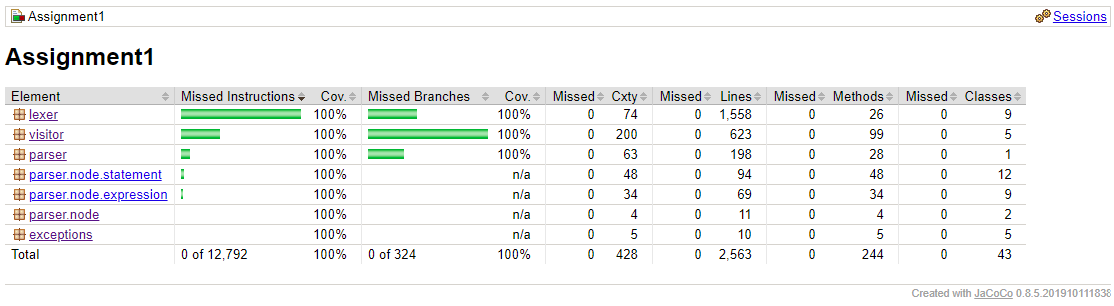
\includegraphics[width=0.9\textwidth]{task1cov.png}
			 			\centering
			  			\caption{Code coverage for task 1}
			  			\label{fig:task1cov}
					\end{figure}
	
	
	A breakdown of these tests can be found in the explanation below.

	\subsubsection{LiteralTest.java}
	
	This testing class contains tests for the constructor method by passing some valid and invalid strings and it is asserted that the correct Literal object or exception is returned. Moreover, tests for the overridden \textbf{equals(Literal)} method were implemented to test all the possible cases.
	
	\subsubsection{ParserTest.java}
	
	This testing class contains tests for the \textbf{parseString(String)} method by passing correct and incorrect strings and then asserting that the expected set of clauses are returned or that a \textbf{SyntaxErrorException} is thrown in case a string is not of the correct format.
	
	\subsubsection{DPLLTest.java}
	
	This testing class includes unit tests to test all the functions used by the DPLL algorithm and it also contains integration tests to make sure that the DPLL algorithm returns the expected results. It should also be noted that in order to test the implementation better, another symbol \quotes{v} was implemented.
	Below, one can find the integration tests performed:
	
	
	\begin{figure}[H]
					\centering
			 			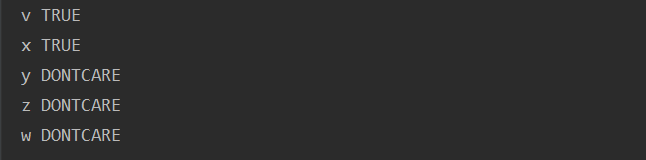
\includegraphics[width=0.7\textwidth]{dplltest1.png}
			 			\centering
			  			\caption{Test result for (x, !y, z)(v, w, y)(v, !x, !z)}
			  			\label{fig:dplltest1}
					\end{figure}
					
	
	\begin{figure}[H]
					\centering
			 			
\includegraphics[width=0.7\textwidth]{dplltest2.png}
			 			\centering
			  			\caption{Test result for (x, y, z)(x, !y)(y, !z)(z, !x)(!x, !y, !z)}
			  			\label{fig:dplltest2}
					\end{figure}
		
		\begin{figure}[H]
					\centering
			 			
\includegraphics[width=0.7\textwidth]{dplltest2.png}
			 			\centering
			  			\caption{Test result for (x)(!x)}
			  			\label{fig:dplltest2}
					\end{figure}
	

		\begin{figure}[H]
					\centering
			 			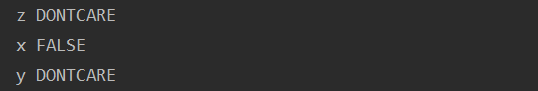
\includegraphics[width=0.7\textwidth]{dplltest4.png}
			 			\centering
			  			\caption{Test result for (!x)(!x,y)(!x,z)}
			  			\label{fig:dplltest4}
					\end{figure}		

			\begin{figure}[H]
					\centering
			 			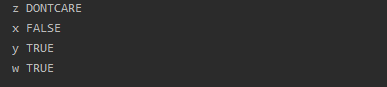
\includegraphics[width=0.7\textwidth]{dplltest5.png}
			 			\centering
			  			\caption{Test result for (!x)(!x,y)(!x,z)}
			  			\label{fig:dplltest5}
					\end{figure}	

				\begin{figure}[H]
					\centering
			 			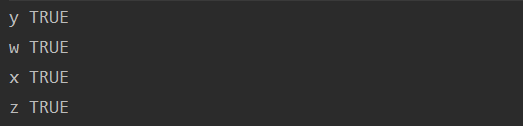
\includegraphics[width=0.7\textwidth]{dplltest6.png}
			 			\centering
			  			\caption{Test result for (w)(x, !y)(z,x)(y,!x)(x, !x)(z, !y)}
			  			\label{fig:dplltest6}
					\end{figure}	

				\begin{figure}[H]
					\centering
			 			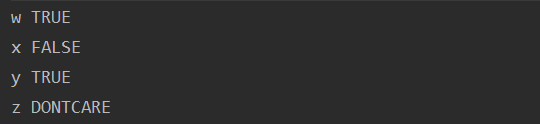
\includegraphics[width=0.7\textwidth]{dplltest7.png}
			 			\centering
			  			\caption{Test result for (x,y)(w)(!x, z)}
			  			\label{fig:dplltest7}
					\end{figure}	
										
				\begin{figure}[H]
					\centering
			 			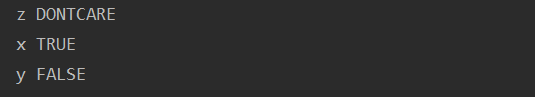
\includegraphics[width=0.7\textwidth]{dplltest8.png}
			 			\centering
			  			\caption{Test result for (x,y)(x,z)(!y, !z)}
			  			\label{fig:dplltest8}
					\end{figure}	
					
				\begin{figure}[H]
					\centering
			 			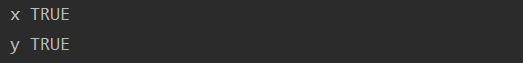
\includegraphics[width=0.7\textwidth]{dplltest9.png}
			 			\centering
			  			\caption{Test result for(x)(!x, y)}
			  			\label{fig:dplltest9}
					\end{figure}						
		
								\begin{figure}[H]
					\centering
			 			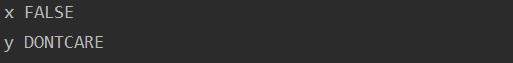
\includegraphics[width=0.7\textwidth]{dplltest10.png}
			 			\centering
			  			\caption{Test result for(!x)(!x, y)}
			  			\label{fig:dplltest10}
					\end{figure}		
					
			\subsection{Practical Applications of SAT}
			
			Just like everything else, anything which is not practical is not very useful. Boolean Satisfiability have been going through improvements throughout the years in order to be used in a practical environment to help in producing a better end product. Moreover, in some
applications, the use of SAT solvers improves performance remarkably \cite{pa3}. The most common applications can be split into 
\begin{itemize}
\item\textbf{product configuration} which involves formulating model lines,  dependencies between components and adhering to customer's restrictions \cite{pa2}.
\end{itemize}
  hardware verification which includes checking the correctness of hardware designs at gate-level and properties related to temporal logic\cite{pa1}.	\\\\
The most well known practical applications include:

\begin{enumerate}
\item \textbf{Combinational Equivalence Checking} : One of the uses of SAT applications checking the equivalence of two circuits, namely, combinational circuits\cite{pa3}. 
\item \textbf{ATPG and SSF} : SAT is used in Automatic Test-Pattern Generation and Single Stuck-at Fault models to be able to identify  fabrication defects in integrated circuits respectively\cite{pa3}. These defects introduce a possibility of of circuit failure and hence, as explained above, SAT helps in making these models better, hence being able to identify and represent the faults ore robustly.
\item \textbf{Bounded Model Checking}: A model checking question asks to show that property always holds while a bounded model checking question asks whether there is a path which contradicts the property, or in other terms, a path which satisfies a failing property. SAT is used in the bounded model checking algorithms which are very common nowadays and are accepted by big companies such as Intel, AMD and IBM\cite{pa1}.
\item \textbf{Planning}: SAT is also used in systems when it comes to planning. In fact, Artificial Intelligence planning was the first push to SAT being used as a practical application\cite{pa3} and from this, a lot of other opportunities were opened for SAT to be used in the areas explained above. This works in a similar way to BMS, hence, increasing the length of paths until the SAT is unsatisfiable. Different types of planning applications include time-tables, air-traffic control and telegraph routing\cite{pa1}. In addition, scheduling of events can also be considered as a practical application of SAT.

	To conclude, as can be seen from the above descriptions, usually SAT algorithms must be able to prove unsatisfiability. The best thing about is as time goes by better variable selection heuristics will be found and the implementation of SAT will be even more efficient and optimized. 

\end{enumerate}

\subsection{How to run}

\begin{enumerate}
\item Go to the directory \quotes{src/main/java}
\item Run \quotes{javac ParserExecutor.java}
\item Run \quotes{java ParserExecutor \textless anyExpression\textgreater}
\end{enumerate}
			
			
		\bibliographystyle{ieeetr}
		\nocite{*}
\bibliography{references}
			
		
			
					
			\end{document}